%%%%%%%%%%%%%%%%%%%%%%%%%%%%%%%%%%%%%%%%%
% Author:	Frederic Afadjigla
% Version: 	1.0
% Date:		23.09.2016
% License:
% CC BY-NC-SA 3.0 (http://creativecommons.org/licenses/by-nc-sa/3.0/)
%
%%%%%%%%%%%%%%%%%%%%%%%%%%%%%%%%%%%%%%%%%

%----------------------------------------------------------------------------------------
%	PACKAGES AND OTHER DOCUMENT CONFIGURATIONS
%----------------------------------------------------------------------------------------

\documentclass[
10pt, % Main document font size
a4paper, % Paper type, use 'letterpaper' for US Letter paper
oneside, % One page layout (no page indentation)
%twoside, % Two page layout (page indentation for binding and different headers)
headinclude,footinclude, % Extra spacing for the header and footer
BCOR5mm, % Binding correction
]{scrartcl}


%%%%%%%%%%%%%%%%%%%%%%%%%%%%%%%%%%%%%%%%%
% Author:	Frederic Afadjigla
% Version: 	1.0
% Date:		23.09.2016
% License:
% CC BY-NC-SA 3.0 (http://creativecommons.org/licenses/by-nc-sa/3.0/)
%
%%%%%%%%%%%%%%%%%%%%%%%%%%%%%%%%%%%%%%%%%

%----------------------------------------------------------------------------------------
%	REQUIRED PACKAGES
%----------------------------------------------------------------------------------------

\usepackage[
nochapters, % Turn off chapters since this is an article        
beramono, % Use the Bera Mono font for monospaced text (\texttt)
eulermath,% Use the Euler font for mathematics
pdfspacing, % Makes use of pdftex’ letter spacing capabilities via the microtype package
dottedtoc % Dotted lines leading to the page numbers in the table of contents
]{classicthesis} % The layout is based on the Classic Thesis style

\usepackage{arsclassica} % Modifies the Classic Thesis package

\usepackage[T1]{fontenc} % Use 8-bit encoding that has 256 glyphs

\usepackage[utf8]{inputenc} % Required for including letters with accents

\usepackage{graphicx} % Required for including images
\graphicspath{{Figures/}} % Set the default folder for images

\usepackage{enumitem} % Required for manipulating the whitespace between and within lists

\usepackage{lipsum} % Used for inserting dummy 'Lorem ipsum' text into the template

\usepackage{subfig} % Required for creating figures with multiple parts (subfigures)

\usepackage{amsmath,amssymb,amsthm} % For including math equations, theorems, symbols, etc

\usepackage{varioref} % More descriptive referencing

%----------------------------------------------------------------------------------------
%	THEOREM STYLES
%---------------------------------------------------------------------------------------

\theoremstyle{definition} % Define theorem styles here based on the definition style (used for definitions and examples)
\newtheorem{definition}{Definition}

\theoremstyle{plain} % Define theorem styles here based on the plain style (used for theorems, lemmas, propositions)
\newtheorem{theorem}{Theorem}

\theoremstyle{remark} % Define theorem styles here based on the remark style (used for remarks and notes)

%----------------------------------------------------------------------------------------
%	HYPERLINKS
%---------------------------------------------------------------------------------------

\hypersetup{
%draft, % Uncomment to remove all links (useful for printing in black and white)
colorlinks=true, breaklinks=true, bookmarks=true,bookmarksnumbered,
urlcolor=webbrown, linkcolor=RoyalBlue, citecolor=webgreen, % Link colors
pdftitle={}, % PDF title
pdfauthor={\textcopyright}, % PDF Author
pdfsubject={}, % PDF Subject
pdfkeywords={}, % PDF Keywords
pdfcreator={pdfLaTeX}, % PDF Creator
pdfproducer={LaTeX with hyperref and ClassicThesis} % PDF producer
}


%----------------------------------------------------------------------------------------
%	HYPHENATION
%---------------------------------------------------------------------------------------
\hyphenation{Fortran hy-phen-ation} % Specify custom hyphenation points in words with dashes where you would like hyphenation to occur, or alternatively, don't put any dashes in a word to stop hyphenation altogether



%----------------------------------------------------------------------------------------
%	Definition of \maketitle
%---------------------------------------------------------------------------------------
\makeatletter         
\def\@maketitle{ 
\begin{center} 
	{\Huge \bfseries \sffamily \@title }\\[1ex] 
	{\Large  \@author}\\[4ex] 
	\@date\\[8ex]
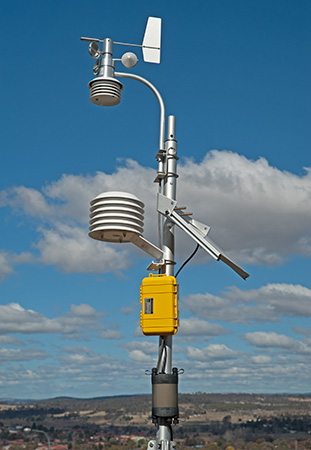
\includegraphics[width = 60mm]{WS}
\end{center}}
\makeatother


%----------------------------------------------------------------------------------------
%	Definition of \maketitle
%---------------------------------------------------------------------------------------
\usepackage{xcolor}
\usepackage{sectsty}
\chapterfont{\color{red}}  % sets colour of chapters
\sectionfont{\color{red}}  % sets colour of sections
\subsectionfont{\color{blue}}  % sets colour of sections

 % Include the structure.tex file which specified the document structure and layout

%----------------------------------------------------------------------------------------

\begin{document}

%----------------------------------------------------------------------------------------
%	TITLE AND AUTHOR(S)
%----------------------------------------------------------------------------------------
\title{{Low Cost Weather Station}} 
\author{\spacedlowsmallcaps{}} 
\date{\today} 
%----------------------------------------------------------------------------------------
%	HEADERS
%----------------------------------------------------------------------------------------

\renewcommand{\sectionmark}[1]{\markright{\spacedlowsmallcaps{#1}}} % The header for all pages (oneside) or for even pages (twoside)
%\renewcommand{\subsectionmark}[1]{\markright{\thesubsection~#1}} % Uncomment when using the twoside option - this modifies the header on odd pages
\lehead{\mbox{\llap{\small\thepage\kern1em\color{halfgray} \vline}\color{halfgray}\hspace{0.5em}\rightmark\hfil}} % The header style

\pagestyle{scrheadings} % Enable the headers specified in this block

%----------------------------------------------------------------------------------------
%	TABLE OF CONTENTS & LISTS OF FIGURES AND TABLES
%----------------------------------------------------------------------------------------

\maketitle % Print the title/author/date block

\setcounter{tocdepth}{2} % Set the depth of the table of contents to show sections and subsections only

\tableofcontents % Print the table of contents

\listoffigures % Print the list of figures

\listoftables % Print the list of tables

%----------------------------------------------------------------------------------------
%	ABSTRACT
%----------------------------------------------------------------------------------------

\section*{Abstract} % This section will not appear in the table of contents due to the star (\section*)


\newpage % Start the article content on the second page, remove this if you have a longer abstract that goes onto the second page

%----------------------------------------------------------------------------------------
%	INTRODUCTION
%----------------------------------------------------------------------------------------
\section{Introduction}

%----------------------------------------------------------------------------------------
%	Setting up your Raspberry Pi
%----------------------------------------------------------------------------------------
\section{Setting up your Raspberry Pi}
\subsection{Prerequisites}
Required are:
\begin{itemize}
	\item \textbf{SD Card}\\
		Recommended is an 8GB preinstalled with NOOBS.
	\item \textbf{Display and connectivity cables} \\
	Any HDMI/DVI monitor or TV should work as a display for the Pi . For best results, use one with HDMI input, but other connections are available for older devices. Use a standard Ethernet cable for internet access.
	\item \textbf{Keyboard and mouse} \\
	Any standard USB keyboard and mouse will work with your Raspberry Pi.
	\item \textbf{Power supply} \\
	Use a 5V micro USB power supply to power your Raspberry Pi. Be careful that whatever power supply you use outputs at least 5V; insufficient power will cause your Pi to behave in strange ways.
\end{itemize}

%----------------------------------------------------------------------------------------
%	Plugging in your Raspberry Pi
%----------------------------------------------------------------------------------------
\subsection{Plugging in your Raspberry Pi}
Before you plug anything into your Raspberry Pi, make sure that you have all the equipment listed above to hand. Then follow these instructions: \\
\begin{enumerate}
	\item Begin by slotting your SD card into the SD card slot on the Raspberry Pi, which will only fit one way.
	\item Next, plug in your USB keyboard and Mouse into the USB slots on the Raspberry Pi.
	\item Make sure that your monitor or TV is turned on, and that you have selected the right input (e.g. HDMI 1, DVI, etc)\\
	\item Then connect your HDMI cable from your Raspberry Pi to your monitor or TV.
	\item If you intend to connect your Raspberry Pi to the internet, plug in an ethernet cable into the ethernet port next to the USB ports, otherwise skip this step.
	\item When you are happy that you have plugged in all the cables and SD card required, finally plug in the micro usb power supply. This action will turn on and boot your Raspberry Pi.
	\item Once your Raspberry Pi has completed the boot process, a login prompt will appear. The default login for Raspbian is username pi with the password raspberry.
\end{enumerate}

%----------------------------------------------------------------------------------------
%	Configuring the Raspberry Pi
%----------------------------------------------------------------------------------------
\subsection{Configuring the Raspberry Pi}

%----------------------------------------------------------------------------------------
%	BIBLIOGRAPHY
%----------------------------------------------------------------------------------------
%\renewcommand{\refname}{\spacedlowsmallcaps{References}} % For modifying the bibliography heading

%\bibliographystyle{unsrt}
%\bibliography{sample.bib} % The file containing the bibliography

%----------------------------------------------------------------------------------------

\end{document}